\chapter{Analyser}
\label{chp:Analyser}
The flash analyser now outputs values at 125Hz, which is a mixture of various light and noise sources. The next step is to create a real-time binary classification algorithm to convert the incoming samples into a logical value: Activity detected, or no activity detected. The detection algorithm should be designed with certain goals in mind:
\begin{itemize}[itemsep=-1ex]
	\item \textbf{High true positive ratio} - The system does not fulfil it's purpose if it is unable to reliably detect bypassing objects.
	\item \textbf{Low false positive ratio} - The system is useless if it classifies everything as activity. This would result in the light being on all the time and therefore, no energy being saved.
	\item \textbf{Fast response time} - If the algorithm manges detect every bypassing person correctly, but it only triggers a detection when the object has already passed the light, then the system does not fulfil its purpose.
	\item \textbf{Low computational complexity} - If the algorithm uses too much calculations per incoming sample, the system would require a strong processor to analyse all incoming data. This makes the system expensive, if it where to eventually get implemented in the real world.
\end{itemize}
This chapter is separated in three parts. The first part shows what signals are received by the photo diode. The second part explains what methods considered to remove unwanted signals from the signal. The final part of this chapter shows what considerations where mode to determine threshold of the binary classifier.

\section{Received signals}
In an ideal world, the dark sensing system only perceives light it emits itself, reflected by the environment. Figure \ref{Signal_properties} shows that this is clearly not the case. Several other factors are influencing the measurements. Equation \ref{eq:Pd_light} has been devised and contains the most common signals the photo diode, $PD$, might receive. Each term of the equation will be discussed briefly while pointing out what the signal looks like.

\begin{figure}
	\centering     %%% not \center
	\subfigure[]{\label{fig:distribution_filteredsum}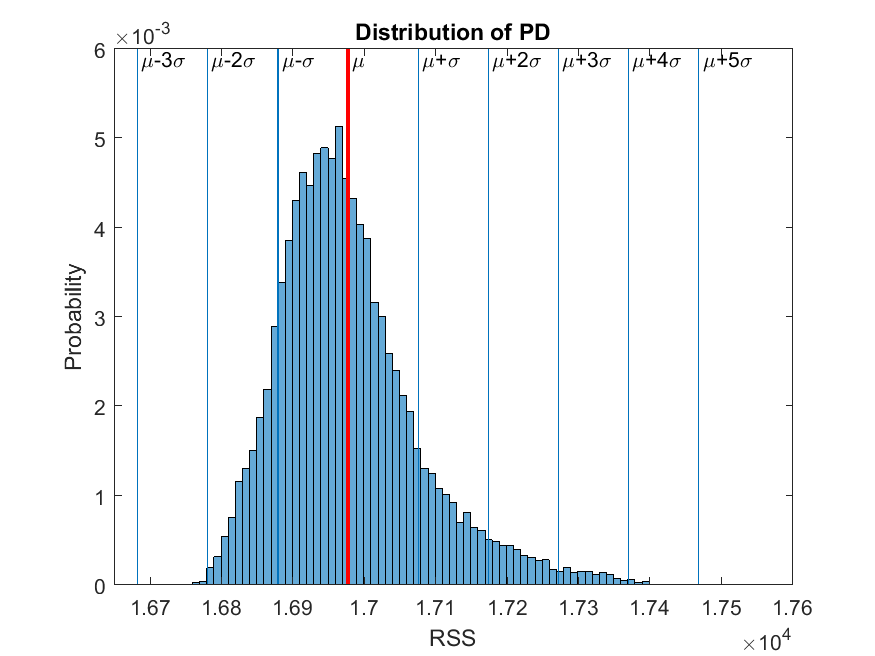
\includegraphics[width=60mm]{pics/distribution_filteredsum.png}}
	\subfigure[]{\label{fig:PSD_original}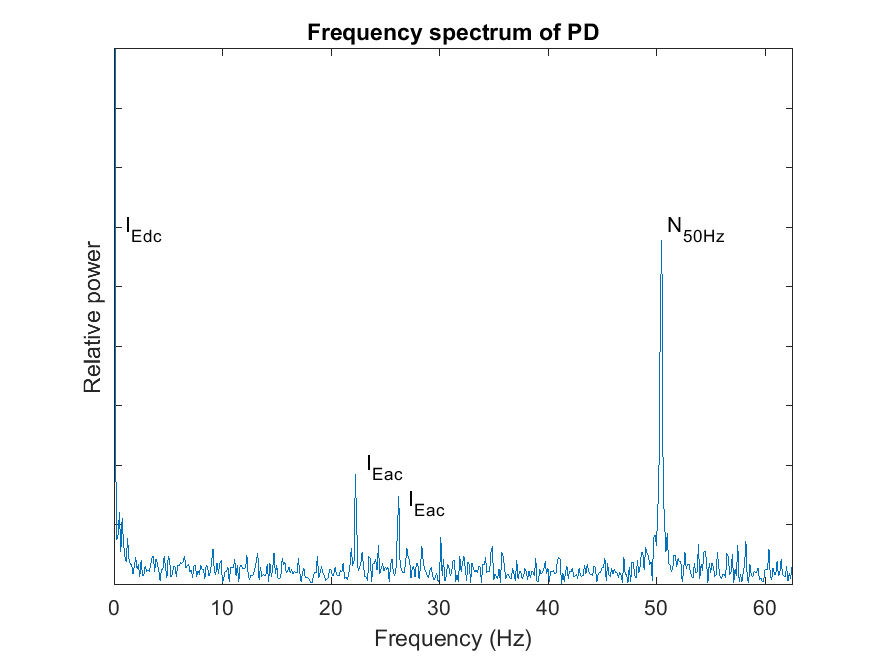
\includegraphics[width=60mm]{pics/PSD_original.png}}
	\caption{Properties of the obtained signal with the the filtered sum method.\label{Signal_properties}}
\end{figure}

\begin{equation}
\label{eq:Pd_light}
PD = I_{L} \alpha + \sum_{i=1}^n I_{Edc_{n}} \beta_{n} + \sum_{i=1}^n I_{Eac{_n}} \gamma_{n} + N_{50Hz} + N(\mu,\sigma^2)
\end{equation}
$I_{L}$ represents the light emitted by the light. This gets multiplied with $\alpha$, which represents the environment from the point of view of the system. These two terms represents the ideal response. The expected frequency of $\alpha$ should lie between $0.2Hz$ and $2Hz$ for by passing pedestrians, as shown in chapter \ref{Model}. The goal of the complete algorithm is to isolate $\alpha$ and detect significant changes in it real-time.

The next term, $\sum_{i=1}^n I_{Edc_{n}}$, represents all constant, but slowly changing light sources in the area. An example of this is moonlight. Moonlight illuminates the surrounding area, but slowly changes over time because moon moves over time, or clouds blocking the moonlight. $\beta_{n}$ represents the environment from the point of view of the moon.
	
$\sum_{i=1}^n I_{Eac{_n}}$ represent all fluctuating light sources in the area. Most lights connected to the power grid fall into this category. They typically turn on and off at 100Hz in Europe. Some of the light produced by these source could reflect of off the environment $\gamma_{n}$ and reach the system and therefore influence the received signal.

Another term in the equation is $N_{50Hz}$, which represents 50Hz noise from the powergrid. As long as the system is connected to the grid, some 50Hz components will be seen in the system. Especially if amplified 1000 times.

the final term, $N(\mu,\sigma^2)$, represents the noise on the measurements not created by the "predictable" sources listed above. This noise originates from the imperfections of the platform and electromagnetic noise in the environment. The exact distribution of the noise is unknown, but its likely to approximate a Gaussian curve. It is therefore represented by its mean ($\mu$) and variance ($\sigma^2$) in the equation.

\section{Filter methods}
The goal of the filters is to get rid of unwanted signals in order to make the detection of $\alpha$ easier. Several digital filters types have been considered, each with different goals mind. The effectiveness (or failure) of each proposed filter will be shown, where possible, with the help of the signals shown in figure \ref{Original_signal}. (a) shows an optimistic case with an original SNR of 18.5. (b) shows a harder case with an original SNR of 10.5. This figure will display the filter working in a much harsher condition.

\begin{figure}
	\centering     %%% not \center
	\subfigure[]{\label{fig:original_good}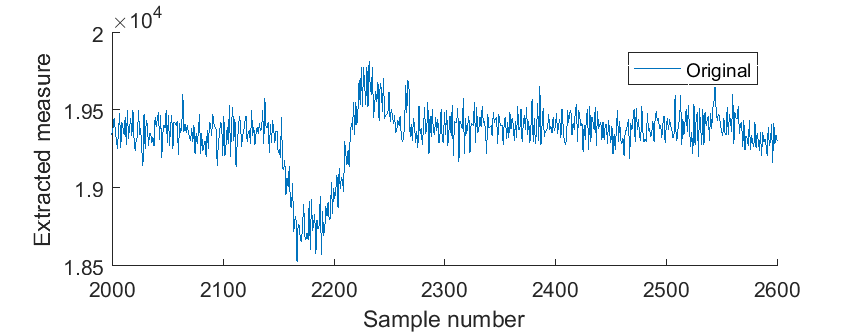
\includegraphics[width=60mm]{pics/Original_good.png}}
	\subfigure[]{\label{fig:Original_bad}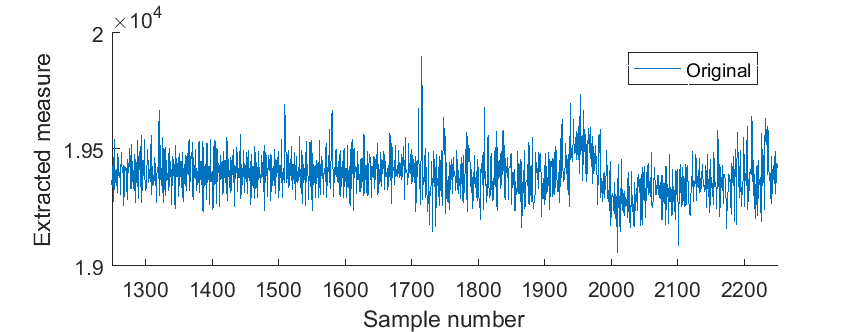
\includegraphics[width=60mm]{pics/Original_bad.png}}
	\caption{Two signals of a person walking underneath the set-up. Figure (a) shows an optimistic case with an SNR of 14.9 and (b) shows a harder scenario with an SNR of 10.5.\label{Original_signal}}
\end{figure}

\subsection{Low-pass filters}
A lowpass filter can be used to remove $I_{Eac{_n}}$ and $N_{50Hz}$ from the measured signal as their frequencies are far removed from the signal we are interested in $\alpha$ (0.1 - 2Hz). Low-pass filters have one big downside for the system. They introduce a delay in the signal when used which is bad for the overall response time. Several filters have been tested. The final result is shown in figure \ref{lowpass_example} and is a second order IIR lowpass with its corner frequency at $5Hz$. Using this filter, the complete $N_{50Hz}$ component of the signal is removed and in most cases, $I_{Eac{_n}}$ is removed as well. We are however unable to grantee the removal of $I_{Eac{_n}}$ because of possible signal aliasing.

Signal aliasing is a phenomenon which occurs if the sample rate $F_{s}$ of a system is too compared to the signal being sampled. If $F_{s}$ is smaller then twice the frequency of then the sampled signal, the signal will appear as another frequency instead, an alias. This frequency is called $F_{alias}$ and can be calculated with equation \ref{Falias}, where $n$ is the closest integer mutiple of $F_{s}$ to the signal being aliased ($F_{Iac}$).

\begin{equation}
\label{Falias}
	F_{alias} = |F_{s} * n - F_{Iac}|
\end{equation}

Almost all lights have a flicker frequency higher than half the sample rate of the system and will therefore alias. In Europe most lights have blink frequencies which are multiples of $100z$ or $200Hz$ (frequency of the power grid) and will therefore show up with alias frequencys of $25Hz$ and $50Hz$. These frequency is can still be removed with the used low-pass filter. There is however no grantee that all lights will blink at a multiple of $50Hz$. In the Americas for example the grid is powered at $60Hz$. The chanse is very high that a light there typically flickers at $120Hz$, which will alias at $5Hz$. This frequency is too low for the low pass filter to remove and will have to be death with in another way (if it occurs).

\begin{figure}
	\centering     %%% not \center
	\subfigure[]{\label{fig:lowpass_good}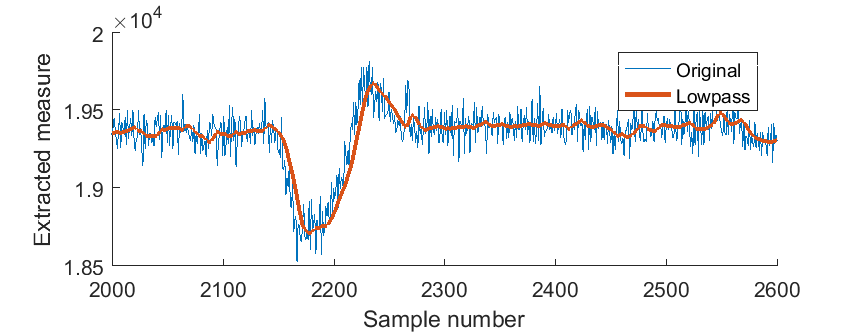
\includegraphics[width=60mm]{pics/lowpass_good.png}}
	\subfigure[]{\label{fig:lowpass_bad}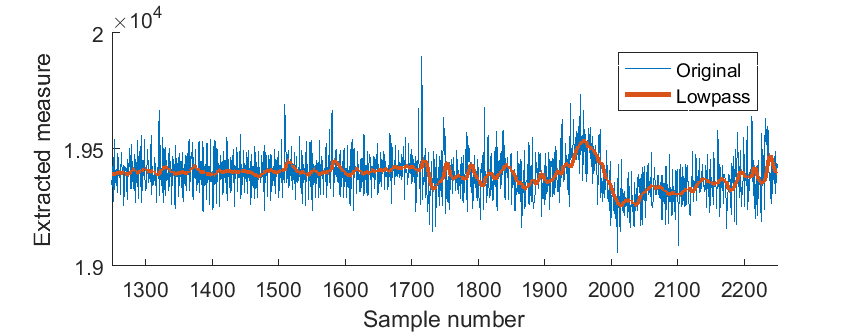
\includegraphics[width=60mm]{pics/lowpass_bad.png}}
	\caption{A lowpass filter ($F_{cutoff} = 5Hz$) applied to the two example signals used to remove $I_{50Hz}$ and $I_{Eac}$. The SNR for signal (a) increased to 27.9 from 14.9 and the SNR of signal (b) increased to 11.7 from 10.5.\label{lowpass_example}}
\end{figure}

\subsection{Highpass filters}
Highpass filters can be used to remove $I_{Edc_{n}}$ from the signal. This is in this specific case very hard as the frequency we are interested in is very close to 0. It works, but it takes the filter a long time to settle if the $F_{Cutoff}$ is chosen too low. Several filters have been tested, and the final result applied to the two test signals is shown in figure \ref{higpass_example}.

\begin{figure}
	\centering     %%% not \center
	\subfigure[]{\label{fig:highpass_good}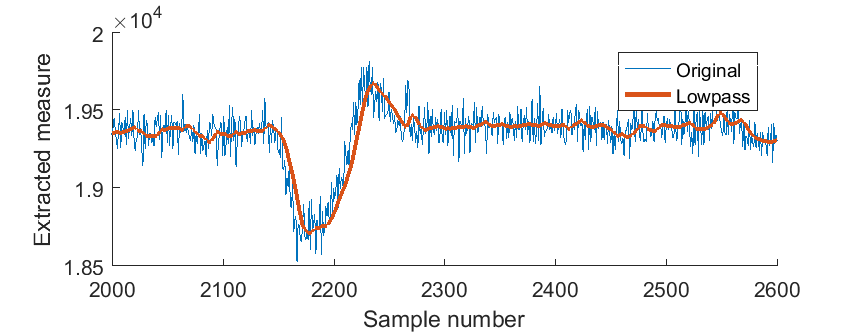
\includegraphics[width=60mm]{pics/lowpass_good.png}}
	\subfigure[]{\label{fig:highpass_bad}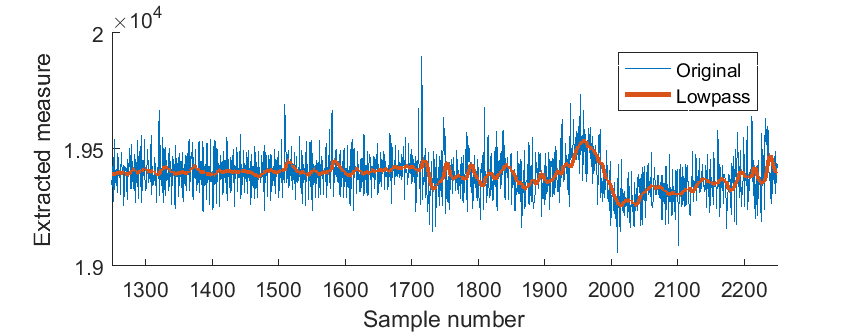
\includegraphics[width=60mm]{pics/lowpass_bad.png}}
	\caption{A highpass filter ($F_{cutoff} = 0.01Hz$) applied to the two example signals used to remove $I_{Edc}$ from the signal. The SNR for signal (a) increased to 30.9 from 27.9 and the SNR of signal (b) increased to 13.3 from 11.7.\label{higpass_example}}
\end{figure}

\subsection{Moving average filters}
A moving average can be used to reduce $N(\mu,\sigma^2)$ and the remaining $F_{allias}$. A moving average is effectively a simple low pass filter with specific frequencies being removed completely at $\frac{F_s}{n}*x$, where $n$ is the number of tabs of the moving average and $x$ any integer greater than 0. Therefore a make shift filter can be created instantly if $F_{alias}$ is known, with $n = \left|\frac{F_{s}}{F_{alias}}\right|$.

$F_{alias}$ could be determined with the help of a Fourier transformation and then filtered away with a make-shift moving average. Yes, the Fourier transform costs a lot of computation power which is against our goal of creating a computationally light algorithm, but the transform wouldn't have to be ran every sample. It is probably good enough to run it once every 10 minutes to check if $F_{alias}$ is detected and/or has changed.

Another advantage the moving average brings is it reduces the noise by a factor $\sqrt{(n)}$, where n is the number of tabs in the filter. It was therefore considered to scale the moving average, based on the current standard deviation of the noise with the help of equation \ref{eq:SNR_movavg}. The presented formula calculates $n$, so that the 

This method has one huge downsides. The first is that a moving average, capable of changing every incoming sample is computational expensive. If $n$ changes, then the full moving average needs to be re-evaluated ($n$ summations, 1 division)) instead of using a simple update rule (1 summation, 1 division). Another downside is that if $n$ gets too large, the response time of the system go down. For these two reasons, the scaling moving average was not implemented in the final algorithm.

\begin{equation}
\label{eq:SNR_movavg}
\frac{signal}{noise} = 1 = \frac{\mu * ss}{T * \frac{\sigma}{\sqrt{n}}} \Rightarrow n = \left(\frac{T * \sigma}{\mu*ss}\right)^2
\end{equation}

\begin{figure}
	\centering     %%% not \center
	\subfigure[]{\label{fig:movavg_good}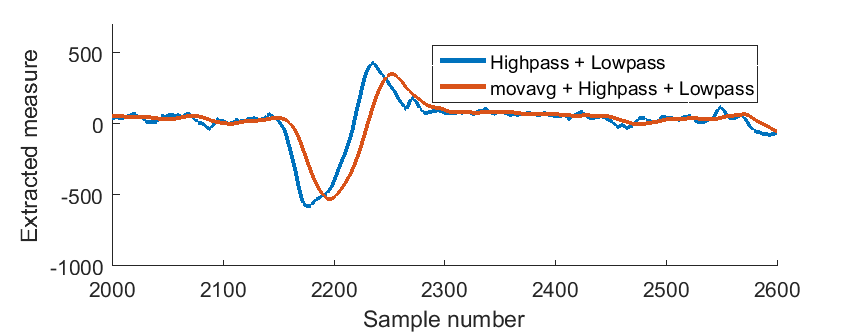
\includegraphics[width=60mm]{pics/movavg_good.png}}
	\subfigure[]{\label{fig:movavg_bad}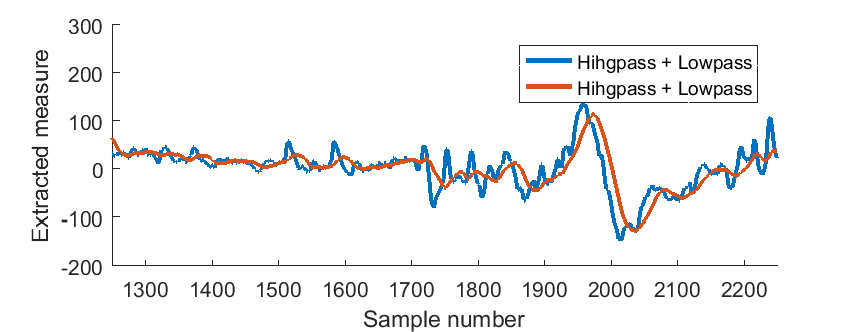
\includegraphics[width=60mm]{pics/movavg_bad.png}}
	\caption{A 28 tabs moving average applied to the two filtered example signals used to remove the remaining $4.5Hz$ component of the signal. The SNR for signal (a) increased to 35.6 from 30.9 and the SNR of signal (b) decreased slightly from 16.6 to 13.3.\label{movavg_example}}
\end{figure}

\subsection{Differential filter}
The differential filter makes use of the fact that the system is not only able to sample when the light is turned on. Instead, It is possible to take samples while the light is turned off, to obtain $PD_{dark}$. This signal represents all the signals in the environment we are not interested in. If this signal is obtained very close to in time relative to $PD$ ($20\mu s$), then we can assume that all fluctuating sources in both, $PD$ and $PD_{dark}$, are equal. It's therefore possible to subtract the two signals, which would result in the filtered signal shown in equation \ref{eq:Pd_light_dark}.

\begin{equation}
\label{eq:Pd_dark}
PD_{dark} = \sum_{i=1}^n I_{Edc_{n}} \beta_{n} + \sum_{i=1}^n I_{Eac{_n}} \gamma_{n} + N_{50Hz} + N(\mu,\sigma^2)
\end{equation}

\begin{equation}
\label{eq:Pd_light_dark}
PD - PD_{dark} = I_{L} \alpha + N(0,\sigma^2 + \sigma^2_{dark})
\end{equation}
There are several downsides to this filtering method. The first is that we are subtracting two separate measures of the same noise signal. This leads to a higher variance on the complete signal and therefore a higher noise level. Another downside of this method is that it does not work properly with the current hardware set-up because the $PD_{dark}$, on its own, is below the sensitivity threshold of the receiver and is therefore unmeasurable, unless there is a lot of stray light in the area.

\subsection{Filter overview}
Several methods for removing unwanted parts of the received signal have been presented and summarised in table \ref{filtersOverview} and result in a better SNR. The final solution implements the lowpass, highpass and moving average with scaling based on $F_{alias}$. Figure \ref{Signal_properties_post_filter} shows the remaining distribution of the noise on the signal.

\begin{figure}
	\centering     %%% not \center
	\subfigure[]{\label{fig:distribution_filteredsum_PostFilters}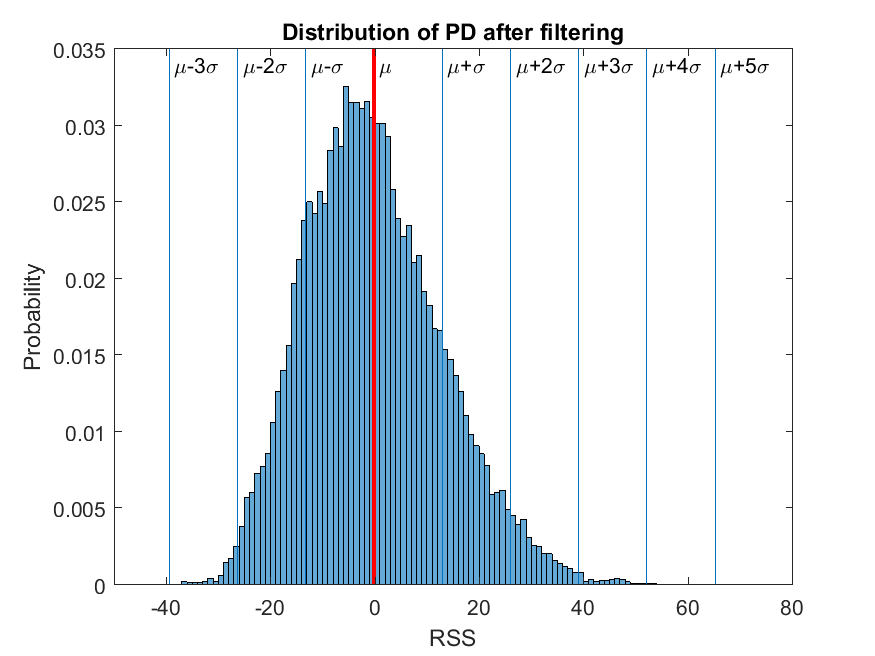
\includegraphics[width=60mm]{pics/distribution_filteredsum_PostFilters.png}}
	\subfigure[]{\label{fig:PSD_PostFilters}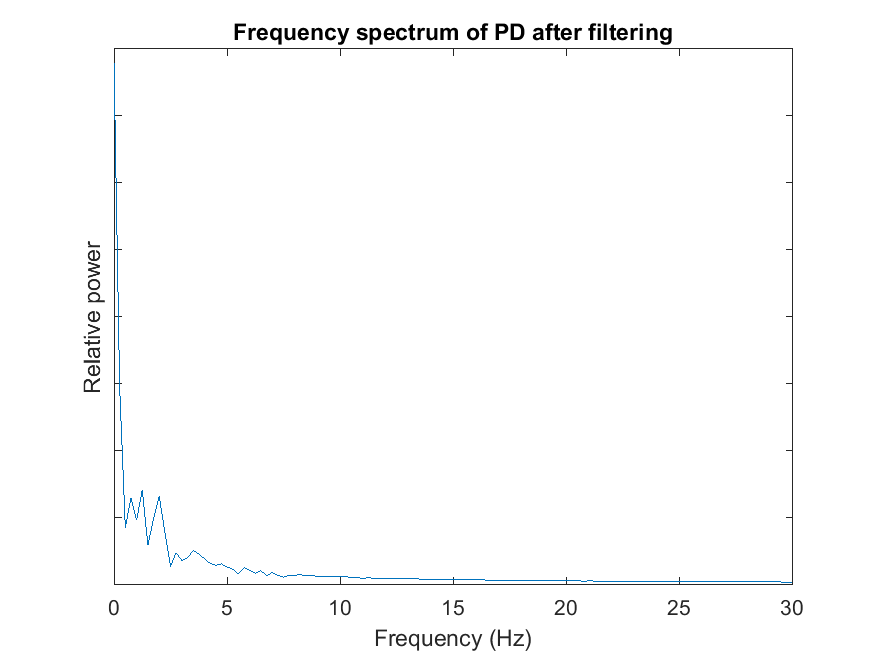
\includegraphics[width=60mm]{pics/PSD_PostFilters.png}}
	\caption{Properties of the signal after filtering. Note that (b) is zoomed in on the frequency axis compared to Figure \ref{fig:PSD_original}\label{Signal_properties_post_filter}}.
\end{figure}

\begin{table}[]
	\hskip-2.0cm
\begin{tabular}{l|lll}
	Filter type                                                        & Goal                                                                                     & Notes                                                                                                                             & In final algorithm? \\ \hline
	Low pass filter                                                    & \begin{tabular}[c]{@{}l@{}}Filter $I_{Eac}$ and \\ $N_{50Hz}$\end{tabular}               & \begin{tabular}[c]{@{}l@{}}Can't guarantee the removal of $I_{Eac}$\\ due to signal aliassing\end{tabular}                        & Yes                 \\ \hline
	High pass filter                                                   & Filter I\_\{Edc\}                                                                        & Takes a long time to settle if a step is received                                                                                 & Yes                 \\ \hline
	\begin{tabular}[c]{@{}l@{}}FFT based\\ moving average\end{tabular} & \begin{tabular}[c]{@{}l@{}}Filter $F_{alias}$ and \\ reduce $N(\mu,\sigma)$\end{tabular} & \begin{tabular}[c]{@{}l@{}}Works, as long as $F_{alias}$ is not too\\ close to $I_{L} \alpha$\end{tabular}                        & Yes                 \\ \hline
	\begin{tabular}[c]{@{}l@{}}SNR based\\ moving average\end{tabular} & reduce $N(\mu,\sigma)$                                                                   & \begin{tabular}[c]{@{}l@{}}Worked, but introduced huge delays for high\\ $\sigma$ and was is computational intensive\end{tabular} & No                  \\ \hline
	$PD-PD_{dark}$                                                     & \begin{tabular}[c]{@{}l@{}}Filter $I_{Eac}$, $N_{50Hz}$\\ and $I_{Edc}$\end{tabular}     & \begin{tabular}[c]{@{}l@{}}Only worked in illuminated environments\\ which made it unreliable to filter $N_{50Hz}$\end{tabular}    & No                 
\end{tabular}
	\caption{Overview of the filter methods described in this section.\label{filtersOverview}}
\end{table}

\section{Detection threshold}
The next step in creating the binary classification algorithm is to determine classifying thresholds or rules. If an extracted value of the set of samples crosses the threshold, then the set gets classified as activity detected. A naive solution to the threshold problem would be to sample a set amount of values when there are no objects in sight. Then, take the maximum and minimum of the sampled values and if the signal ever moves out of the range of the found values, activity is detected. Even though this might work consistently in a dark room (lab environment with no lights), it fails to work in a more realistic environment. If a "dirty" device in the environment turns on then this could increase the noise level in the environment. which would lead to false detections.

This failed method shows that the threshold needs to be able to adaptable based on the noise in the environment. Two other algorithms have been considered, which are possibly capable of adjusting their thresholds in an intelligent manner.

\subsection{Standard deviation based threshold}
The first method is based upon the standard deviation. We could set the detection threshold based on the current measure on $\sigma$. Several real-time algorithms are known to calculate rolling $\sigma$, the standard deviation over all samples which have passed by. This measure gives a good estimate of the noise in the environment until something happens. If an object passes by for example, an "extreme" change in the signal will occur and the rolling standard deviation will be deluded with non-noise samples, ruining the noise estimate.

This issue can be solved by using a moving standard deviation. This method only uses the most recent $m$ samples to obtain $\sigma$ and bases it's detection threshold on this value. This means, that if an event occurs, the algorithm only remembers it for $m$ samples. By using a system with only a short-term memory, we can create an flexible system which automatically adjust to permanent changes in the environment.

Using the idea of moving $\sigma$, we can create a simple threshold algorithm with equation \ref{Zscore}. This equation calculates the z-score for the most recent sample out of the filter section $\overline{X}[i]$ and compares it with threshold value $T$. Then if z is greater than $T$ or smaller than $-T$, it triggers a detection. $\sigma_i$ and $\mu_i$ in this equation represent the a moving mean and standard deviation over the most recent $m$ samples at $i$.

\begin{equation}
	\label{Zscore}
	z_i = \frac{\overline{X}_i - \mu_i}{\sigma_i}
	\qquad
	(-T < z_i < T) \rightarrow detection 
\end{equation}
Figure \ref{fig:InfluenceOfD_noD} shows the described algorithm in action. It can be seen that the bypassing person is detected at sample 2962. This is a good result, but rather slow, especially since we are able to see the signal rise from sample 2875. The reason why the algorithm does not trigger a detection is because the threshold ($T * \sigma$) has risen slightly due to the variance on being increased, which is caused by change in the signal itself. This problem can be solved in a very simple way. Prevent $\sigma$ from being updated before an event happens. This can be achieved by adding a small delay of $d$ samples between X and the threshold. An example of this is shown in Figure \ref{InfluenceOfD_withD}, where the event is detected at 2879 samples, which is 83 samples (0.66 seconds) earlier than the previous result.

\begin{figure}
	\centering     %%% not \center
	\subfigure[]{\label{fig:InfluenceOfD_noD}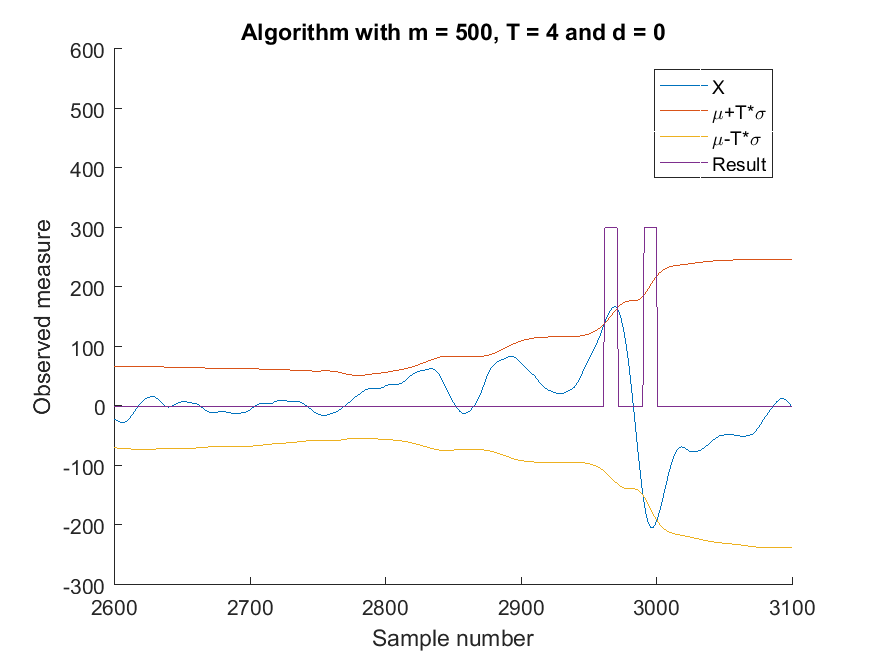
\includegraphics[width=60mm]{pics/InfluenceOfD_noD.png}}
	\subfigure[]{\label{fig:InfluenceOfD_withD}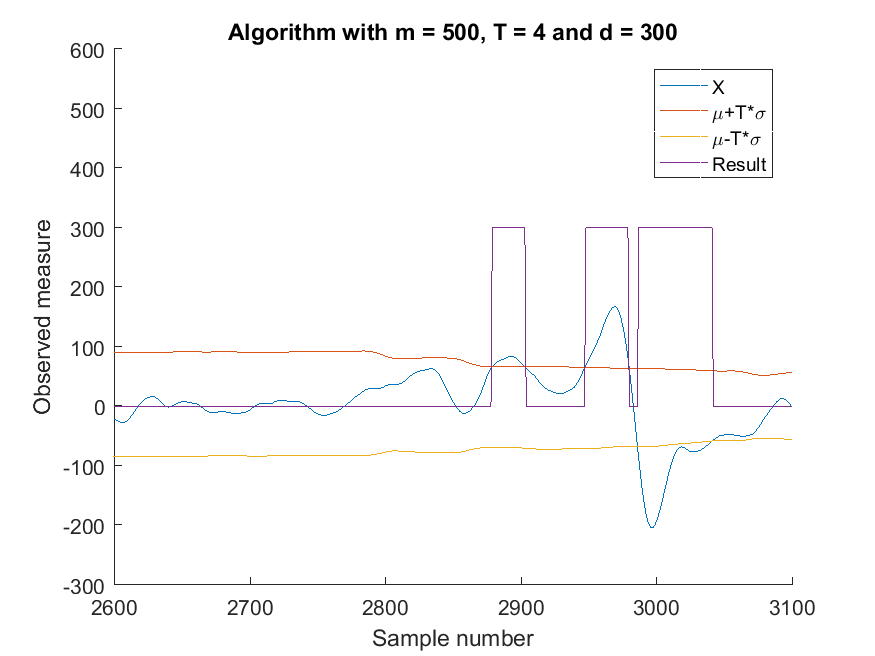
\includegraphics[width=60mm]{pics/InfluenceOfD_withD.png}}
	\caption{Working of the algorithm visualized with and without delay ($d$) between the standard deviation ($\sigma$) and the signal ($X$).\label{fig:InfluenceOfD}}
\end{figure}

Several other parameters where added to further improve the classification algorithm. The first one is to add a linear offset $k\cdot\sigma$ to the detection threshold, because the noise distribution of the device is not balanced, meaning that there are more outliers on one side of the mean, than there are on the other side. This can be seen in Figure \ref{fig:distribution_filteredsum_PostFilters}. If we where to move $\mu$ slightly more to the right with a factor $0.75 \sigma$, then the distribution would be more balanced (all samples lie between $\pm 3.5\sigma$) which results in a better overall sensitivity.

Another improvement we can make is to not look at only one observation of $\overline{X}$, but $L$ consecutive ones instead. If we then only trigger a detection if $l$ out of $L$ samples cross the threshold then it might be possible to run the algorithm with a smaller $T$ and therefore detect more events. 

Equation \ref{Zscore_improved} shows a mathematical representation of the threshold algorithm. A graphical overview of the complete algorithm (including the filter section) can be seen in Figure \ref{fig:algtot}.

\begin{equation}
\label{Zscore_improved}
\sum_{i = -L}^{0} \Bigl\lfloor{\frac{\overline{X}_i + k\cdot\sigma_{i-d} - \mu_{i-d}}{T \cdot \sigma_{i-d}}} \Bigr\rfloor \geq l \rightarrow detection 
\end{equation}


\subsection{Variance based threshold}
The other threshold method considered for classifying several consecutive samples is to only look at the variance of the signal. In Figure \ref{fig:InfluenceOfD_noD} it was observed that the standard deviation changes rapidly if an event occurs. If we wanted, we could simply calculate the variance ($\sigma^2$) of the signal and check if it exceeds a certain threshold. If it does, we trigger a detection. This method can be summarized with equation \ref{eq:varr_based_T}.

\begin{equation}
\label{eq:varr_based_T}
\sigma^2_i > T \rightarrow detection
\end{equation}
This method has similar problems as previously described methods:
\begin{itemize}[itemsep=-1ex,topsep=0pt]
	\item A static threshold, $T$, is unable to cope with changes in the environment noise.
	\item A rolling variance as threshold would be deluded by the events, and therefore be deceptively high.
\end{itemize}
Similar problems ask for similar solutions. It was therefore chosen to use a moving variance over $m$ samples as measure and a delayed moving variance, delayed in time by $d$ samples, as threshold. This results in a variable threshold with a short-term memory which is able to deal with adjustments in the environment. This method can be improved even further by adding the variables $l$ and $L$ as discussed in the previous subsection. By checking $l$ out of $L$ samples cross the threshold, we can afford to use a lower $T$ and detect even smaller changes. A mathematical representation of this algorithm is given in equation \ref{varr_improved}. A graphical representation of the full algorithm (including filters) is shown in figure \ref{fig:algtotstd}.
\begin{equation}
\label{varr_improved}
\sum_{i = -L}^{0} \Bigl\lfloor{\frac{\sigma^2_i}{T\cdot\sigma^2_{i-d}} }\Bigr\rfloor \geq l \rightarrow detection 
\end{equation}

\begin{figure}
	\centering     %%% not \center
	\subfigure[]{\label{fig:algtot}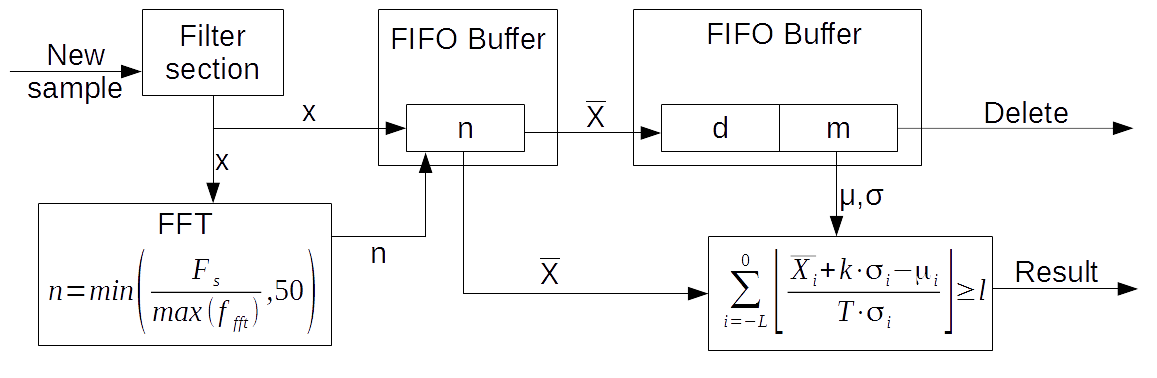
\includegraphics[width=120mm]{pics/ThresholdAlgorithmOverview_double_FIFO.png}}
	\\
	\subfigure[]{\label{fig:algtotstd}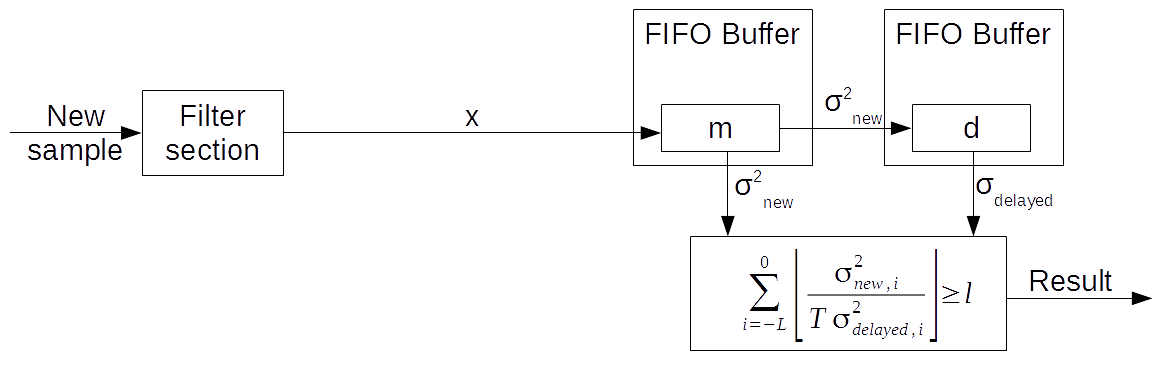
\includegraphics[width=120mm]{pics/ThresholdAlgorithmOverview_STD.png}}
	\caption{The two versions of the algorithm. (a) shows the absolute verionion and (b) shows the standard deviation version.\label{fig:fullAlgorithm}}
\end{figure}

\section{Conclusion}
